%  Copyright (c)  2005  EDF-EADS-PHIMECA.
%  Permission is granted to copy, distribute and/or modify this document
%  under the terms of the GNU Free Documentation License, Version 1.2
%  or any later version published by the Free Software Foundation;
%  with no Invariant Sections, no Front-Cover Texts, and no Back-Cover
%  Texts.  A copy of the license is included in the section entitled "GNU
%  Free Documentation License".
\section{Introduction}

This document is part of Open TURNS' documentation. Its aim is to introduce the global methodology for the quantification of uncertainties by a model-based approach, and the methods proposed by Open TURNS to carry out the different steps of such a study. Indeed, even if each industrial study exhibits some particularities, a common framework composed of four steps is proposed.

\begin{itemize}

\item[$\bullet$] {\bf Step A}: {\em specification of the case-study: uncertainty sources, model and criteria} \\
  The objective is to identify the sources of uncertainty, and the major characteristics of interest of the system studied that are influenced by these sources.
\item[$\bullet$] {\bf Step B}: {\em quantification of the uncertainty sources } \\
  The characteristics of the uncertainty sources are determined in a deterministic or probabilistic framework.
\item[$\bullet$] {\bf Step C}: {\em uncertainty propagation} \\
  A numerical method is carried out to compute the uncertainty of the system's characteristics of interest.
\item[$\bullet$] {\bf Step C'}: {\em ranking of the sources of uncertainty / sensitivity analysis} \\
  Chosen indicators are used to rank the uncertainty sources with respect to their impact on the uncertainty of the system's characteristics of interest.

\end{itemize} \vspace{2mm}

The first part of this document briefly presents each step, and illustrates the key points through a realistic -- even though simplified -- example.

In the second part of the document, the focus is placed on the methods that an analyst may use in Open TURNS to carry out steps B, C and C'. For each method, a synthetic form is given to highlight:

\begin{itemize}

\item[$\bullet$] the mathematical principles,
\item[$\bullet$] the position of the method in the global methodology,
\item[$\bullet$] some basic recommendations on when and how to use (and not to use) the method,
\item[$\bullet$] some key bibliographic references.

\end{itemize}

For the practical side i.e. the use of these functions in Open TURNS Textual User Interface, the User is refered to the  \otrefext{OpenTURNS_UserManual_TUI}{TUI User Manual} and \otrefext{OpenTURNS_UseCasesGuide}{TUI Use Cases Guide}.

\subsection{Presentation of the flood example}
\par

Suppose that the industrial study concerns a dyke built along a river to protect an industrial facility from floods. For the industry that runs this facility, a risk exists: even if the dyke would have been high enough to contain the major floods of the last century, one does not know if the protection will be sufficient to face the next flood. For instance, meteorological events vary from year to year and are thus considered random, at least given our current knowledge in this scientific field. Therefore, an uncertainty study becomes valuable to ensure risk control (the dyke should be high enough to limit the risk of inundation) and economical optimization (the construction and maintenance cost increase with the dyke height, which should consequently not be either under or over-dimensioned).

\newpage

\section{Global methodology of an uncertainty study}

\subsection{Step A: specification of the case-study}

The first step of an uncertainty study can be roughly described as "the definition of the problem". This may seem obvious, but starting an uncertainty study requires an analysis of some key issues -- the foundations that will ensure that the industrial goals have been correctly translated in mathematical terms.

\subsubsection{Variables of interest, model and input variables}

In our framework, a {\em variable of interest} denotes a scalar variable on which the uncertainty is to be quantified. A {\em model} denotes a mathematical function that enables the computation of a set variable of interest, being given several {\em input variables} on which the User may have data and/or expert/engineering judgement. The basis of the uncertainty study is the following mathematical equation:
$$
\underline{y} = h \left( \underline{x},\underline{d} \right)
$$
where:
\begin{itemize}
\item[$\bullet$] $\underline{y} = \left( y^1,\ldots,y^{n_y} \right) \in \mathbb{R}^{n_y}$ is a vector that regroups the variables of interest,
\item[$\bullet$] $h$ denotes the model,
\item[$\bullet$] $\underline{x} = \left( x^1,\ldots,x^{n_x} \right) \in \mathbb{R}^{n_x}$ denotes the vector of input variables of the model on which uncertainties are to be studied,
\item[$\bullet$] $\underline{d}= \left( d^1,\ldots,d^{n_d} \right) \in \mathbb{R}^{n_d}$ denotes the vector of input variables of the model treated as certain (uncertainties are negligible/neglected, or a penalized value is used).
\end{itemize}

\begin{center}
  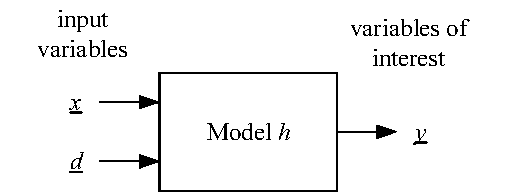
\includegraphics[scale=0.8]{flow.pdf}
\end{center}

\paragraph{Illustration on the flood example}
\par

A key variable to be studied is the annual maximum water level; in addition, one may also want to consider the annual cost including damage caused by possible floods and  maintenance of the dyke. Therefore, two {\em variables of interest} $\underline{y} = \left( y^1,y^2 \right)$ can be studied: $y^1$ denotes the annual maximum water level, and $y^2$ denotes the overall annual cost. $y^1$ can be evaluated via more or less complex hydrological models, the main input factors being the river flow and some characteristics of the river bed (such as Strickler's coefficient to represent the friction i.e. the bed roughness). $y^2$ requires in addition an economical model to assess the costs (systematic maintenance and damages repair).

Some of the models input variables are uncertain: the river flow and bed's characteristics are naturally variable from year to year, and damage cost may not be well known. They are therefore part of $\underline{x}$, even if some of them may be put in $\underline{d}$ by using penalized value (e.g. a maximal damage cost or a "worst possible" Strickler's coefficient). This last approach could be chosen if too scarce information is available on these sources of uncertainty.

Note that every model is a simplified view of reality, which introduces another source of uncertainty in the analysis. Thus, one has to keep in mind the importance of a compromise between model uncertainty (complex models usually offer a more accurate evaluation of the variable of interest) and input variables uncertainty (complex models may involve much more uncertain factors on which information has to be available).

\subsubsection{Criteria of the uncertainty study}

Now that the general context has been staged, one major question is still to be addressed before moving to the core of the uncertainty study. The variable(s) of interest for the User are known to be uncertain, and this uncertainty is to be quantified; but what exactly could we or should we use to measure uncertainty? Open TURNS' methodology proposes deterministic and probabilistic criteria that meet many industrial cases requirements.

\paragraph{Deterministic criteria}
\par

In a deterministic context, one may want to assess the range of possible values of $\underline{y}$, that is to say a subset $D_y \subset \mathbb{R}^{n_y}$ in which we are {\em sure} to find $\underline{y}$. In the following, we will refer to this type of uncertainty measurement as a {\em deterministic criterion}; Open TURNS proposes methods that can be used to estimate the minimum and the maximum of a variable of interest.

This approach is the easiest to understand from a conceptual point of view, easier anyway than the probabilistic approach that we will now address. But we will see in step C that it is not always the less demanding approach in terms of CPU time.

\paragraph{Probabilistic criteria: probability of exceeding a threshold / failure probability, and quantile}
\par

Most of the methods proposed in Open TURNS use a probabilistic framework. In such a context, the vector $\underline{y}$ of variables of interest is seen as a mathematical object called {\em random vector}, usually noted in capital letters $\underline{Y}$. Roughly speaking, this means that one associates a probability to each interval (and more generally to each subset of values). Note that in such an approach, the range of possible values of $\vect{Y}$ may be infinite e.g. the water level in our flood problem may be somewhere between 0 and $+\infty$, even if very large values will be associated to probabilities that are extremely close to zero.

The most complete measure of uncertainty when dealing with a random vector is the {\em probability distribution}. One way to characterize a probability distribution is the following function $F_Y$, called {\em cumulative distribution function}:
$$
F_Y \left( y^1,\ldots,y^{n_y} \right) = \mathbb{P} \left(  Y^1 \leq y^1,\ldots, Y^{n_y} \leq y^{n_y} \right)
$$

In an uncertainty study, one may want to assess the value of the cumulative distribution function at least in certain points. More precisely, focus may be placed on the following quantities.

\begin{itemize}
\item[$\bullet$] {\em Probability of exceeding a threshold}: the aim is to assess the probability of the event $\mathcal{D}=$ "the variable of interest $Y^i$ exceeds a threshold important for the industrial goals at stakes (e.g. safety)":
  $$
  \mathbb{P} \left( Y^i > \textrm{threshold} \right) = 1 - F_{Y^i} \left( \textrm{threshold} \right)
  $$
  In industrial applications concerning structural reliability, one often talks of "failure probability", term that will also be used in Open TURNS' documentation. By convention (also derived from the field of structural reliability), the event "threshold exceeded" is often re-written as:
  $$
  \mathcal{D}_f= \big\{ \vect{x} \in \mathbb{R}^{n_x} \ \big| g\left( \underline{x},\underline{d} \right) < 0 \big\}
  $$
\item[$\bullet$] {\em Quantiles}:  the aim is to assess the threshold that a variable of interest may exceed with a probability equal to a given value. For $\alpha \in ]0,1[$, the quantile of level $\alpha$ of a scalar variable of interest $Y^i$ is defined as follows:
    $$
    q_{Y^i}(\alpha) \ \textrm{is the scalar such that}\ \mathbb{P} \left( Y^i \leq q_{Y^i}(\alpha) \right) = F_{Y^i} \left( q_{Y^i}(\alpha) \right) = \alpha
    $$
\end{itemize}

These criteria are very rich in terms of industrial meanings. But their assessment may be sometimes quite demanding in terms of CPU time (step C) and/or knowledge on the sources of uncertainty (step B). This is why in some applications, practitioners may be interested in more simple probabilistic criteria.

\paragraph{Probabilistic criteria: central dispersion}
\par

The {\em expectation}/{\em average value} $\mu_{i}$ and {\em variance} $\sigma^2_{i}$ of a variable of interest $Y^i$ are defined as follows:
$$
\mu_{i} = \mathbb{E} \left( Y^i \right), \ \sigma^2_{i} = \mathbb{E} \left[ \left( Y^i - \mu_{i} \right)^2 \right]
$$
Exception made of very particular cases, these two quantities are not sufficient to compute the probability of exceeding a threshold, or a quantiles. But they provide an "order of magnitude" of uncertainty: the standard deviation $\sigma_{i}$ (square root of the variance) -- normalized by the average value $\mu_{i}$ in order to remove scale effects -- is an indicator of the {\em dispersion} of the variable of interest $Y^i$. Values distant from $\mu_{i}$ are more likely if $\sigma_{i}$ is large.

\begin{center}
  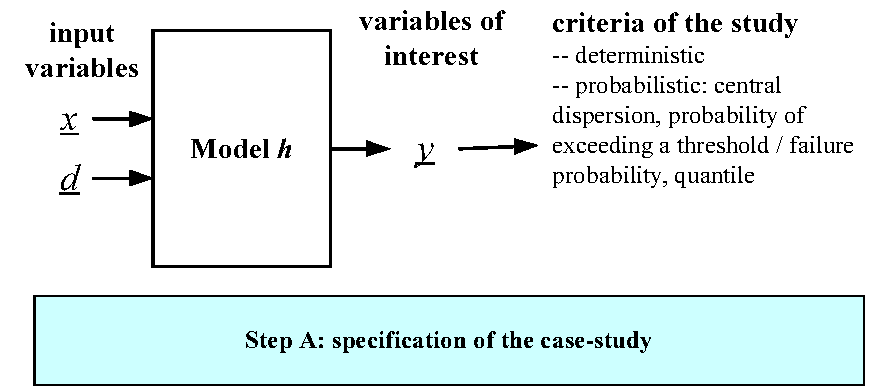
\includegraphics[scale=0.8]{flow2.pdf}
\end{center}

\paragraph{Illustration on the flood example}
\par

In our flood example, practitioners may be interested is the probability of a flood over a year. Since $Y^1$ denotes the annual maximum water level:
$$
\mathbb{P} \left( Y^1 > \textrm{dyke\;height} \right) = 1 - F_{Y^1} \left( \textrm{dyke\;height} \right)
$$
Another probabilistic quantity of interest would be the 99\%-quantile of the variable of interest $Y^1$, that is to say the level of water that is exceeded only 1 time per century on average (probability of exceeding the threshold equal to 1\%). Note that here, one has in mind very low probabilities. But if the description of the methods proposed in Open TURNS often place the focus on low probabilities assessment -- which yields specific difficulties -- it is obviously possible to use these methods in order to adress "non-rare" events.

The value of these indicators (probability of flood and quantiles) is relevant {\em only} if one is able to provide an accurate probabilistic model of the uncertainty sources (e.g. the river flow and the bed's characteristics), problem that will be addressed in step B. If information on the uncertainty sources is scarce or difficult to collect, a first uncertainty study could focus on the expectation and standard deviation of the variable $Y^1$, which will bring some first useful -- even though limited -- informations on uncertainty.

\subsection{Step B: quantification of the  uncertainty sources}

Once step A has been carried out, the next step is to define a model to represent the uncertainties on the vector $\underline{x}$. The methods to be used depend mainly on the type of criteria chosen (deterministic or probabilistic) and on the information available (statistical datasets and/or expert/engineering judgement).

\paragraph{Deterministic criteria}
\par

In a deterministic framework, the range of possible values has to be determined for each component of the uncertainty sources $\underline{x}$.

\paragraph{Probabilistic criteria}
\par

In a probabilistic framework, the vector $\underline{x}$ of uncertainty sources is seen as a random vector denoted by $\underline{X}$. The uncertainty study then requires to assess the probability distribution of $\underline{X}$.

The first question that has to be investigated concerns the possible dependencies between uncertain variables. Common physical phenomenon may link several components of vector $\underline{X}$; then obtaining an information on $X^i$ would change our knowledge of $X^j$. If such dependencies are suspected, a multi-dimensional analysis is required in order not to bias the results of the uncertainty study. In case of independence, a uni-dimensional analysis for each $X^i$ is sufficient.

In this version, Open TURNS proposes a way of building a multi-dimensional probability distribution of $\underline{X}$ in two sub-steps.

\begin{itemize}

\item[$\bullet$] First, a uni-dimensional analysis has to be carried out for each uncertainty source $X^i$. The methods proposed by Open TURNS are described below.

\item[$\bullet$] Second, some measures of the dependencies between the sources of uncertainty are to be determined through expert/engineering judgement or statistical tools provided by Open TURNS. The measures used by Open TURNS are correlation coefficients; the underlying mathematical tools are so-called "copulas".

\end{itemize}

In the uni-dimensional case, the way to build a probability distribution depends on the available data.

\begin{itemize}

\item[$\bullet$] Sometimes, the only available information is an expert/engineering judgement based on an analysis of the underlying physics, feedback of experience from other studies, dedicated literature, etc. Then, Open TURNS proposes a list of {\em parametric models} that describe various types of uncertainty thanks to a small number of parameters; these parameters can be chosen according to expert/engineering judgement.

\item[$\bullet$] Suppose now that datasets are available: several measurements of the variable $X^i$ have been carried out previously. Then, one may use again a {\em parametric model}, but this time with the help of statistical tools provided by Open TURNS in order to choose the most relevant model, estimate its parameters and validate the resulting model. Anyway, there still exists a risk of choosing a non-relevant parametric model, which may result in an inaccurate uncertainty study. The User may avoid this risk by choosing a  {\em non-parametric model} proposed by Open TURNS: the result is only "data-driven" -- which ensures robustness -- but the number of data required is much larger than for a parametric model, especially if the uncertainty study focus on rare events.

  Note that whatever the method used to build a probability distribution (parametric or non-parametric), two phases can be distinguished: the construction of the model, and its critical analysis regarding the objectives of the study (based on data or expert/engineering judgement). This second phase should focus on the "important" parts of the probability distribution: for instance, if the criterion of the study is a rare quantile, a special attention has often to be paid to extreme values of the uncertain variables. If the criterion deals with central dispersion, the requirement on extreme values are less important.

\end{itemize}

\begin{center}
  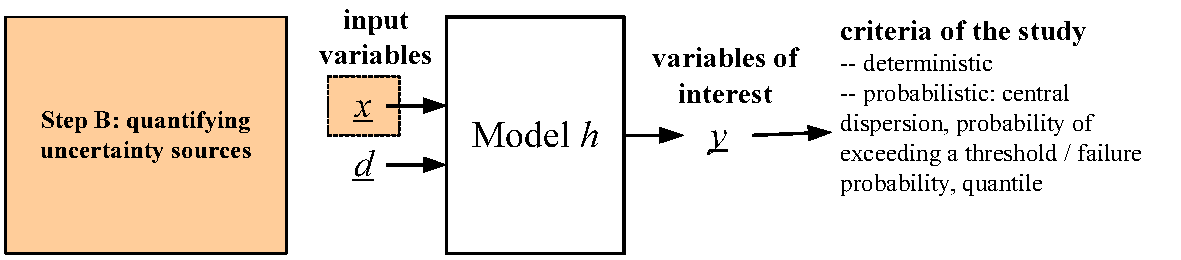
\includegraphics[scale=0.8]{flow3.pdf}
\end{center}

\paragraph{Illustration on the flood example}
\par

In a deterministic framework, note that the upper limit for the river flow is always relative: whatever "realistic" value is proposed, one has to be aware that there is still a residual risk of exceeding this limit.

If a probabilistic framework is considered, some uncertainty sources can be reasonably assumed independent: there is no physical reason that may justify a dependancy between the river flow and Strickler's friction coefficient  (knowing the flow of arriving water does not give any information on the state of the river bed). But if several uncertain variables characterize the river bed (e.g. Strickler's coefficient and some indicators of topography), the question of dependency should be investigated in order not to false the results of the study, even if it is an additional source of complexity.

Finally, note that some relationships between the variable of interests and some uncertain variables are monotonic. For instance, the maximum value of the water level will be reached for the highest possible value considered for the river flow, since a non-decreasing relation intuitively exists between these variables. Therefore, studying a high quantile of the water level requires a good confidence in the probabilistic model of extreme river flow values.

\subsection{Step C: uncertainty propagation}

Now that the analysis on the uncertainty sources has been carried out, the next goal is to translate the model chosen in step B in terms of uncertainty on the variables of interest via the relation:
$$
\underline{y} = h \left( \underline{x},\underline{d} \right)
$$
The method to be used depends on the criteria of the study, and on some characteristics of the model $h$.

\paragraph{Deterministic criteria}
\par

In this situation, range of values have been determined for $\underline{x}$. Finding the minimum and maximum values of $\underline{y}$ is quite easy if the model $h$ is monotonous with respect to $\underline{x}$ (one only has to consider the boundary values of $\underline{x}$). But in a more general context, this is a potentially complex optimization problem. Open TURNS proposes a simplified approach based on design of experiments to estimate extreme values of $\underline{y}$.

\paragraph{Probabilistic criteria}
\par

Step B has provided the probability distribution of $\underline{X}$. The objective is then to assess some characteristics of interest of the distribution of $\underline{Y} = h \left( \underline{X},\underline{d} \right)$: probability of exceeding a threshold, quantile, or expectation and variance. Open TURNS proposes a set of relevant methods for each of these quantities.

\begin{itemize}

\item[$\bullet$] For the assessment of expectation/variance or threshold exceeding probability, Open TURNS proposes both approximation methods (numerically efficient whatever the CPU cost of a run of $h$, but only valid if the analyst can justify some properties of $h$ e.g. regular, close to linear, etc.) and robust sampling methods (no assumption is made on $h$, but CPU-cost becomes a more critical issue).

\item[$\bullet$] For the assessment of  a quantile, Open TURNS proposes a sampling method.

\end{itemize}

\begin{center}
  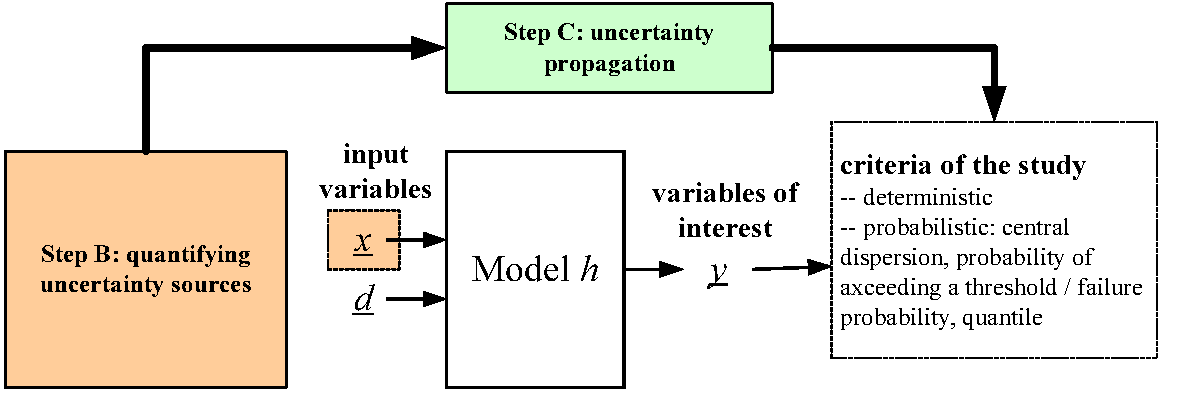
\includegraphics[scale=0.8]{flow4.pdf}
\end{center}

\paragraph{Illustration on the flood example}
\par

In a deterministic framework, the computation of extremum values is facilitated by the fact that some relationships between the variable of interests and some uncertain variables are monotonic, as mentioned above: the maximum value of the water level will be reached for the highest possible value considered for the river flow.

In a probabilistic framework, the complexity of the hydrological model $h$ plays an important role in the propagation method to be chosen. If a simple model with a low CPU cost is used, robust sampling methods are the most natural candidates. Otherwise, approximation methods and/or accelerated sampling methods may be attractive. Note that one does not have to choose a {\em unique} method: cross-validating the results by using several propagation methods may be fruitful!

\subsection{Step C': Ranking uncertainty sources / Sensitivity analysis}

In a probabilistic framework, a better understanding of uncertainties can be achieved by analysing the contribution of the different uncertainty sources to the uncertainty of the variables of interest. For each couple "criteria of the study / propagation method used in step C", post-treatment procedures are proposed by Open TURNS in order to rank the uncertainty sources.

It is important to note that an uncertainty study rarely stops after a first processing of steps A, B, C and C', and the last step then plays a crucial role. Indeed, the ranking results highlight the variables that truly determine the relevancy of the final results of the study. If the uncertainty model of some of these variables has been chosen a bit roughly in step B e.g. because of time constraints or any practical difficulties, collecting further informations on these meaningful sources would be a relevant move to refine the analysis.

\begin{center}
  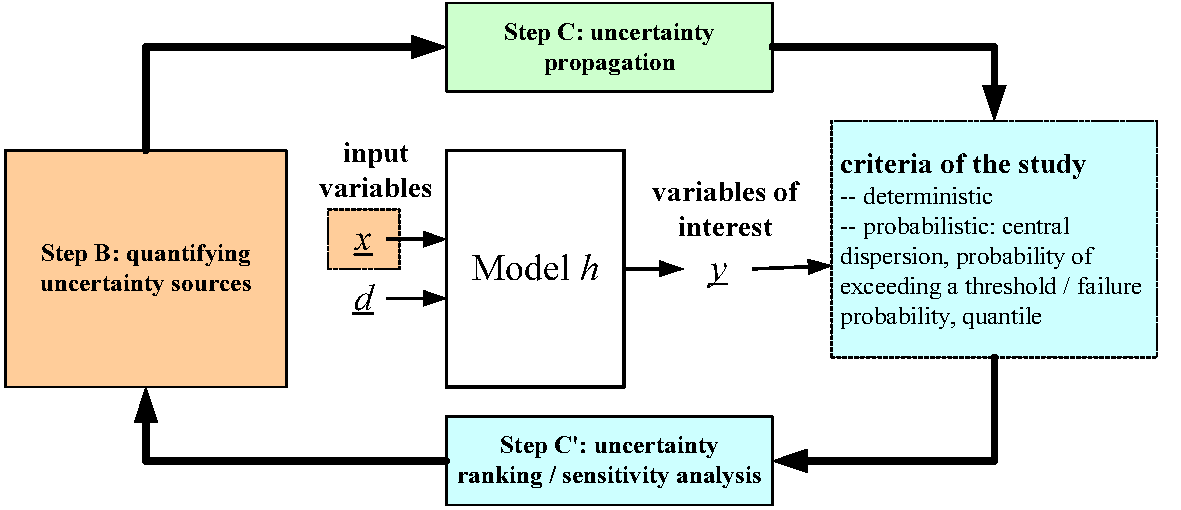
\includegraphics[scale=0.8]{flow5.pdf}
\end{center}

\paragraph{Illustration on the flood example}
\par

It is important to note that the result of the uncertainty ranking is strongly linked to the type of criterion considered. For instance, suppose that the central dispersion of the annual maximum water level is studied. Suppose also that the river flow is pointed out by uncertainty ranking as the most important uncertain variable, the other ones having almost a negligible impact. However, it would be dangerous to say without further investigation that this would be the same if the focus is shifted towards extreme values of the variable of interest (high quantile or rare probability). it is quite possible that the role of bed's roughness uncertainty will be increased since extreme values of the water level may come only from the conjunction of a high flow {\em and} a high roughness.

